\chapter{Realization}
In the following chapter, we describe the realization of the software system. In section \ref{sec:structure}, we give an overview of the core components and how they interact with each other. 
In section \ref{sec:additional}, we describe additional components. Figure \ref{fig:componentsOverview} shows an overview of the core components. Additional components from section \ref{sec:additional} are omitted.


\begin{figure}[h]
    \centering
    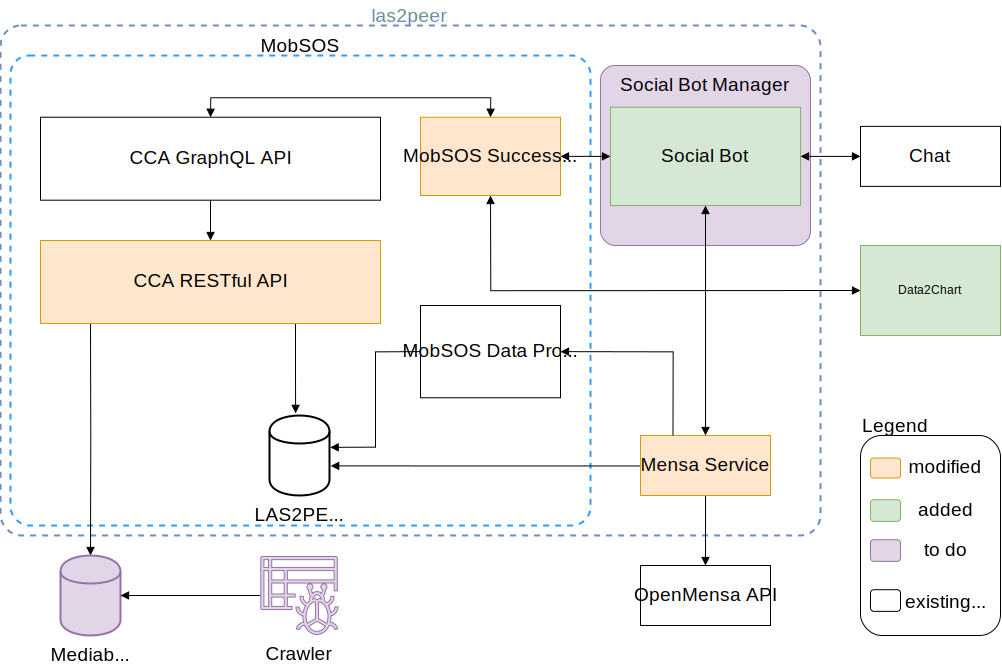
\includegraphics[width=\linewidth]{realization/components_overview.png}
    \caption{Overview of the different components}
    \label{fig:componentsOverview}
\end{figure}

\section{Structure}\label{sec:structure}
The system consists of three major components: the \emph{Social Framework}, the \emph{Mensa Service}\footnotemark and the \emph{MobSOS} services. 
The resulting bot model can be seen in \ref{fig:botmodel}
\footnotetext{\href{https://github.com/rwth-acis/las2peer-Mensa-Service}{las2peer Mensa Service}}
\subsection{Social Bot Framework}
The Social Bot Framework is used to model and deploy the \emph{mensabot}. The mensabot is created in the space of the Social Bot Framework.
\begin{figure}[h]
    \centering
    \includegraphics[width=\linewidth]{realization/botmodel.png}
    \caption{Bot model inside the canvas}
    \label{fig:botmodel}
\end{figure}

The bot model is created on the canvas of the frontend. The resulting model is shown in Figure \ref{fig:botmodel}. The frontend also serves to write the intents, which will be used to train an NLU model for intent recognition. 
The bot should be able to be added to group channels. The bot should act as a quiet agent listening to mentions and filter out the rest of the conversations.
A mention has the following form \texttt{@botname}, where \emph{botname} represents the username that the bot has in the Slack channel.


\subsection{MobSOS services}
The MobSOS services include the MobSOS Data Processing, MobSOS Success Modelling , MobSOS CCA GraphQL, MobSOS CCA REST services.

\subsubsection{MobSOS CCA GraphQL and REST}
The MobSOS CCA backend service has access to three different databases. First, the MobSOS CCA service can access the food reviews, which are stored inside the las2peer database of the Mensa Service. Second, the system can access \emph{Mediabase} data, which contains data from reviews, made outside of the las2peer system. 
% This data could be collected by a crawler bot, which searches Google and Twitter for reviews of the canteen. Those two databases provide the information quality factors of the MobSOS success model.
Third, the CCA service can also access monitoring data generated by the Bot and the Mensa Service. 
% Those monitoring messages provide the system quality factors of the MobSOS success model.


\subsubsection{MobSOS Data Processing}
The MobSOS Data Processing service collects logs from the Mensa service and the MobSOS Success Modelling service. 
Logging data in MobSOS can be done by using the listing \ref{lst:logging}
\begin{lstlisting}[caption=Example use of a MonitoringEvent,captionpos=b,label={lst:logging}]
    Context.get().monitorEvent(
        MonitoringEvent.SERVICE_CUSTOM_MESSAGE_X, data
    );
\end{lstlisting}.
The MonitoringEvent \texttt{enum} provides different events which are logged in the network. An overview of the different monitoring events can be found on GitHub \footnote{\href{https://github.com/rwth-acis/mobsos-data-processing/wiki/Built-In-Monitoring-Events}{GitHub: MonitoringEvent}}. 
Each service can use its own events by using the \texttt{MonitoringEvent.CUSTOM\_MESSAGE\_X}, where \emph{X} is a number between 1 and 99. 
Those \texttt{data} variables contains generic JSON data. This data provides information about how community members are using the service.
To monitor messages in the service, the service needs to be started using the \texttt{--observer} flag.
The data is stored in the MobSOS MySQL database under the \texttt{MESSAGE} table. The table contains a column \texttt{REMARKS} which is used to store the JSON data.

\subsubsection{MobSOS Success Modelling}
The MobSOS Success Modelling service is used to make the visualizations of success factors and measures defined by the community. The service stores success models per group and per service. 
The groups reflect the las2peer \emph{GroupAgent} and the services reflect the \emph{ServiceAgents} in the las2peer network.
The success model contains the six MobSOS dimensions.
\begin{lstlisting}[ caption=Example of a success model,language=XML ]
<SuccessModel name="Name of success model" 
    service="your.service.name@version">
    <dimension name="name of dimension 1">
        <factor name="Name of factor">
            <measure name="No Factors or Measures yet"/>
        </factor>
    </dimension>
    .
    .
    .
    <dimension name="name of dimension n">
        <factor name="Name of factor">
            <measure name="No Factors or Measures yet"/>
        </factor>
    </dimension>
</SuccessModel>
\end{lstlisting}
Each of these dimensions includes a list of success factors.
Each factor contains a list of success measures. The success measures are stored in a separate file called \emph{Measurement Catalog}. Each measure contains a \texttt{query} element which contains the SQL query and a \texttt{visualization} element which contains information about the visualization.
\begin{lstlisting}[language=XML, caption= example of a Measure Catalog]
<Catalog>
    <measure name="Your measurement">
        <query name="countOfMessageX">
            SELECT COUNT(*) as number 
            FROM monitoringTable.MESSAGE
            WHERE EVENT =  'SERVICE_CUSTOM_MESSAGE_X' 
            AND SOURCE_AGENT = '$SERVICE$'
        </query>
        <visualization type="KPI">
            <operand name="countOfMessageX" index="0"/>
        </visualization>
    </measure>
   .
   .
   .
</Catalog>
\end{lstlisting}
Three types of visualization are supported
\begin{itemize}
    \item Value
    \item Chart
    \item KPI
\end{itemize}
The MobSOS Success Modelling service uses the GraphQL API to get the data defined in the query and then uses the Data2chart service to visualize the data as a picture of a chart in base64 encoding. This encoded picture is then sent back to the las2peer bot manager.

The measure definition was extended with a \texttt{database} element which is part of the query and which gives additional information about which database the query should be executed on. The attributes for the \texttt{database} element are \texttt{name} and \texttt{dbSchema}. The name identifies the database on the GraphQL server. The \texttt{dbSchema} describes which schema should be used.
Both of these attributes can be omitted. In this case, when the GraphQL query is prepared the default database and default database schema are used, which are \texttt{las2peer} and \texttt{LAS2PEERMON} respectively.
This allows the community to visualize data from any database supported by the GraphQL service.

\subsection{Google Charts API}
Google Charts API\footnotemark is an API that provides visualizations for database data. The data, which should be visualized needs to be wrapped inside a JavaScript class called \texttt{DataTable}, which represents a two-dimensional table with rows and columns, where each column has a datatype.
A new column can be added using the \texttt{DataTable.addColumn} function, which takes the type and name as input. An example can be seen in Listing \ref{lst:gglCharts} from the Google Charts API documentation\footnotemark[\value{footnote}].

\begin{lstlisting}[caption=Example use of the DataTable class,captionpos=b,label={lst:gglCharts}]
var data = new google.visualization.DataTable();
data.addColumn('string', 'Topping');
data.addColumn('number', 'Slices');
data.addRows([
	['Mushrooms', 3],
	['Onions', 1],
	['Olives', 1], 
	['Zucchini', 1],
	['Pepperoni', 2]
]);
\end{lstlisting}
\footnotetext{\href{https://developers.google.com/chart}{Google Charts API}}

The visualizations are rendered as SVGs in the browser, but can be the PNG file can be accessed by make a http call with the \texttt{getImageURI} as image URI parameter. 

\subsection{Data2chart}
This service was written by me\footnotemark in order to render google charts as an image which could be sent to the chatbot and visualized in the chat. This service was created as an alternative to the MobSOS query visualization service which did not provide the option to render the chart as an image. 
\footnotetext{\url{https://github.com/lakhoune/image-renderer}}
The service is written in NodeJS and uses an NPM library called google-charts-node\footnotemark.
\footnotetext{\url{https://www.npmjs.com/package/google-charts-node}}
This module creates an html file which loads the google charts and then renders that html file in a headless browser \footnotemark and returns the resulting image.
\footnotetext{\url{https://www.npmjs.com/package/puppeteer}}
The MobSOS success modelling service calls this service if a bot is requesting a visualization. It includes the data for the graph in a post request which has the following form:

\begin{lstlisting}
POST  http://localhost:3000/ HTTP/1.1
content-type: application/json

{
    "data": [...],
    "chartType":"BarChart",
    "options":{
        "title":"Chart title",
        "hAxis":{
            "title":"Axis title"
        }
    },
    "clean":true 
}
\end{lstlisting}

\subsection{Mensa Service}
The Mensa Service provides information about the community to the bot. This information includes: canteens, dishes and reviews. The Mensa service logs MobSOS data which is later used to get insights about how the Mensa community uses the service.

Initially this service stored Mensa related information in the shared node storage. The service was modified to use its own database. This was mainly due to issues when getting access to Envelopes which often lead to a Envelope Access denied exception and inconsistencies in the shared storage. Using a database also allows us to persist reviews and make them available to display MobSOS related success visualizations.
The Mensa service was also extended to use the OpenMensa API \footnote{\url{https://openMensa.org/}}. This allows us to use information about canteens all over Germany and even neighbouring countries.
This change also means that we no longer need to crawl the website of the Studierendenwerk \footnote{\href{https://www.studierendenwerk-aachen.de/}{Studierendenwerk Aachen}}, which is prone to errors if they change their website. 

\section{Social Bot}

The bot acts as an interface between the user, and the las2peer backend services. The bot is called \emph{Mensabot}.
Chat messages from users are sent to the bot manager service. 
The bot manager uses a RASA server for intent recognition. 
The RASA server also extracts the name of the Mensa and the city in which it is located as possible intent entities from the user input.

Certain actions, like requesting the menu or a visualisation , trigger a service call to the \emph{Mensa Service}, or the \emph{Success Modelling Service}.
The services get access to the user message.  
The services also get access to context information like the intent and the entities that were recognized by the RASA server.
Furthermore they also get access to meta-information from the chat platform like the channel\_id of the Slack channel or the email address of the chat user. 
The email address is used to store user information in the service. This is done in a static HashMap, which maps email addresses to context information. The context information for a particular user is a \texttt{JSON} object containing itself generic \texttt{Object}s referenced by a \texttt{string} key. 
Storing this information inside the service is important for a REST service, as the context will not be provided on a next service request.

\subsection{Communication with the Mensa Service}
The first feature, which was implemented was querying the menu for a specific canteen. 
The process is depicted in Figure \ref{fig:getMenu}.
\begin{figure}[h]
    \centering
    \includegraphics[width=8cm]{realization/bot/menu.png}
    \caption{Get Mensa related information}
    \label{fig:getMenu}
\end{figure}
The user asks the bot for the menu at a specific canteen. 
This then triggers a bot action calling the las2peer Mensa service. 
Possible intent entities which are recognized at this step are the \emph{name} of the canteen and the city in which the canteen is located.
If the name of the canteen is not recognized, the bot will ask  the user again to specify it. The city name can be omitted. In this case it is possible that multiple canteens match the name provided by the user. If this is the case the bot will provide a list of all matching canteen names and then ask the user to choose one of the canteens from the list. The list is saved in context, so that the user can provide a number and the service can then select the appropriate canteen from the list.
After fetching the menu the bot asks the user if they would like to set the city in which the canteen is located as their default city. If the user types yes, then this city is saved in the context of the user. On further requests this information can be helpful to extract the right canteen if more canteen names are possible. 
I chose to set the default city instead of the default canteen students from one Mensa community might visit different canteens in the same city and less likely to change cities. 

Next the review process was implemented as a question-based dialogue. An example can be seen in figure \ref{fig:addReview}.

\begin{figure}[h]
    \centering
    \includegraphics[width=\linewidth]{realization/bot/review.png}
    \caption{Add a review}
    \label{fig:addReview}
\end{figure}

The bot starts by asking the user to which canteen he went and what category of dish they had. If the user did not specify a canteen, but had previously asked for the menu than the Mensa service gets the canteen from the \texttt{ContextInfo}. 
The provided intent entities are the name of the canteen and the category of dish (e.g. Klassiker/ Vegetarisch) 
The bot then extracts the dish from the menu and ask the user if the canteen and dish were correctly selected. Currently, dishes are only extracted by dish category, by using simple string matching. Furthermore, the dish categories need to be provided in the same way that they are mentioned on the menu. In our case, this means that they need to be provided in German.
If the user confirms the selection then the process continues. The canteen and dish are stored in the context. If the selection was wrong the bot asks the user to retry specifying the canteen and dish. The context is reset to the previous step in this case, this also includes removing the dish and canteen from the user context in the service.
After the user has confirmed that the right canteen and dish were indeed selected, the bot continues to ask the user how many stars (out of 5) the user would give their meal. 
The bot then asks the user to add a comment to the review. The user can either add a comment or not. If the user types \emph{no} into the chat the bot recognizes this as a rejection intent and adds a review without comment.
Both of these features should be implemented as soon as possible. The reason for this is to allow the collection of food reviews and service logs, which can then be evaluated at a later time.
This also allows the first phase of the evaluation to take place (see Chapter \ref{cha:eval}).
The food reviews will be done in private chat with the bot. The menu query should be available both in private chat and in channels, given that the SBF is already extended to allow for mentions.

\subsection{Communication with the MobSOS Success Modelling service}

The next feature, which was implemented was the visualisation of success measures. Users can request visualisations by stating that they want to visualize something.
This triggers the visualization routine of the bot.

The bot starts by asking providing the name of a success \emph{measure}. Alternatively the user can also ask the bot to list all measures of the success model.
If the user asked to list measures, they can then choose one of the measure name from the list. 
The measure name is passed on to the Success Modelling service. The service then gets the success success model for the community. In our case this is done by using the default group name and default service name, but they can be specified too.
If a group different to the default group is chosen, then the service checks if the chat user is part of the las2peer group. It is important to note here that the email address needs to be assigned to an Agent in the network. This can be done by using the las2peer frontend. Groups can also be managed under \emph{AgentTools} on the frontend.   
 An example can be seen in figure \ref{fig:visualReq}.
\begin{figure}[h]
    \centering
    \includegraphics[width=\linewidth]{realization/bot/visual.png}
    \caption{Requesting a visualisation}
    \label{fig:visualReq}
\end{figure}

After discussions with my supervisor, we decided not to add the ability to formulate queries directly with the bot. The GraphQL service is only used internally by the MobSOS Success Modelling service. The success measures are predefined using a tool like the MobSOS evaluation centre. The measures contain a \texttt{tags} attribute which can be used to add keywords to a measure. The bot uses entity extraction to extract possible tags from a user message, which then are used in the success modelling service to find the right measure for the visualization in the measure catalog and success model.

The Bot Service communicates with the MobSOS Success Modelling system in order to get visualisations of the success model. The bot sends the resulting visualisations to the user in chat.
Furthermore, it can also be used to modify the success model of the community. 
Finally the success modelling will be implemented. Users should be able
to modify the success model in chat. Therefore, an update routine needs to be implemented, which is started at the recognition of a specific intent.
The bot is modelled with the help of the Social Bot Framework frontend canvas and deployed on the las2peer social bot manager service.


\section{Additional services}\label{sec:additional}
Some additional systems were deployed or added during my work.

\subsection{Mensa Guide}
The Mensa Guide service is a frontend to the las2peer Mensa service. It provides basic functionalities like getting the menu for canteens in Aachen, making reviews and uploading pictures for dishes.  

\subsection{MobSOS evaluation Center}
The MobSOS evaluation Center is a service which communicates with the MobSOS backend services. It provides a range of functionalities. Those include: contact management and group management. 
It also allows community members to editing existing success models or create new ones.
Furthermore it also provides visualizations for the measures of the success model, which it gets from the MobSOS query visualization service.

\subsection{MobSOS query visualization service}
The MobSOS query visualization service is a las2peer service which can be used to make visualizations of data in a database. It also allows users to add new database and store SQL queries. The MobSOS Evaluation Center uses this service to get the visualizations for success measures.





% \subsection{MobSOS CCA}
% The MobSOS CCA system needs to be extended such that the success model data can be visualized and sent as a picture to the user. Therefore, the Google Charts API will be used in combination with an HTML renderer, which will render the visualizations which were produced by the Charts API and send them back as a PNG to the Bot Service.

This measure is recognized by the bot to run the visualisations. Additionally, templates will be available, which are to be run when specific intents are recognized, such that the query visualisations can be done in an intuitive way.




% \begin{figure}
%     \centering
%     \includegraphics[height=0.45\textheight]{realization/chat_mockup.png}
%     \caption{Example use of community Service with the Bot}
%     \label{fig:chatMockup}
% \end{figure}

% \begin{figure}
%     \centering
%     \includegraphics[height=0.45\textheight]{realization/visual_req.png}
%     \caption{Example of a chat interaction with the Bot}
%     \label{fig:visualReq}
% \end{figure}